\documentclass{article}
\usepackage[final]{nips_2017}
\usepackage[utf8]{inputenc} % allow utf-8 input
\usepackage[T1]{fontenc}    % use 8-bit T1 fonts
\usepackage{hyperref}       % hyperlinks
\usepackage{url}            % simple URL typesetting
\usepackage{booktabs}       % professional-quality tables
\usepackage{amsfonts}       % blackboard math symbols
\usepackage{nicefrac}       % compact symbols for 1/2, etc.
\usepackage{microtype}      % microtypography
\usepackage{graphicx}
\usepackage{subcaption}
\usepackage{wrapfig}
\usepackage{array}
\title{Spoken Command Recognition}

\author{
  Thomas Karpati \\
  Department of Computer Science\\
  Stanford University\\
  \texttt{tkarpati@stanford.edu} \\
}

\begin{document}
% \nipsfinalcopy is no longer used

\begin{center}

\includegraphics[width=3cm, height=0.7cm]{CS230}
\end{center}

\maketitle

\begin{abstract}
  Interactions with agents in the world has increasingly been using
  voice commands, allowing users to interact without the use of a
  terminal input such as when they are not in close proximity, are
  otherwise physically occupied, or users such as children who
  are illiterate and cannot use standard computing interfaces which
  would require the ability to read. In the simple case such an agent
  would need to be able to recognize basic commands to perform
  tasks. We propose a 2D convolutional and recurrent network model for
  this task.
\end{abstract}

\section{Introduction}
Speech recognition is allowing more accessible interactions with
agents. Deep learning systems have enabled improved speech
recognition accuracy through sequential models, which increases the
accessibility of system to a wider variety of users, and allows
interactions with agents who may not be in physical proximity of the
user. Often the inputs to these sequential models is the spectrogram
representation of an audio waveform. This is a representation which
converts the time domain audio waveform into a multidimensional basis
space for segments of time over a sliding window. The result of this
is a multidimensional representation of the audio waveform during a
specified period of time. As these are accumulated over time, this can
be seen as a two dimensional representation of the audio waveform. Our
algorithm explores applying two dimensional network architectures to
a traditional sequential model for speech recognition processing as a
more hybrid model for performing speech recognition.

The inputs to our algorithm are audio waveforms. We have 10 known classes of
commands and two additional classes which are an unknown command class
and a no spoken word class. Our network requires an initial processing
step to generate the spectrogram of the waveform as input to the
network. In addition to our proposed hybrid network, we also explore
performing complete end-to-end processing in our network from the raw
audio waveform without any pre-processing steps. 

\section{Related work}
There are several approaches to the speech recognition
problem. Dominant approaches involve use of recurrent networks which
take the sequential nature of the audio as it progresses through time
into account. These vary from those with simple recurrent cells to
larger more complex bi-directional recurrent cells that process large
segments of time at once\cite{amodei2016deep}. Other approaches to the
command recognition
problem involve use of both 1D and 2D convolutional
networks\cite{oxerin-baseline, arik2017convolutional} as well
as simple fully connected dense networks over the spectrogram of the
data.

Both of these approaches have their advantages and drawbacks. The
fully connected dense and two dimensional convolutional
networks can extract significant features across the entire space of
the input to the network by using the entire time and frequency
information available\cite{hinton2012deep}. The 2D convolutional
network is able to extract
features from both across time and across frequencies by applying
network structures from image processing to the
spectrogram\cite{sainath2015convolutional}. This
approach does indirectly ignore the sequential nature of the data (but
can take
this into account by the relative weights of the connections to
different parts of the spectrogram) however the exact position of the
utterance in question needs to known so that the utterance can be
located properly within the time frame that is being looked at.

The recurrent networks take the sequential nature of speech into
account. These networks have shown to be highly effective in speech
recognition, and typically use the spectrogram as the input feature
transformation to the input of the network. Effective speech
recognition systems will typically also employ bidirectional recurrent
cells for encoding the speech data\cite{zhang2017hello}. The drawback
here is that
bidirectional networks will impact the latency for command
detection. While effective for speech-to-text or translation domains,
keyword and command recognition system are latency sensitive, and thus
the bidirectional nature of these recurrent networks are
impractical. Also, systems which implement 1D convolution before the
recurrent cells, while taking the frequency domain into account, do
not fully allow for convolution across the frequencies. Even systems
that only convolve in two dimensions may not be taking invariance into
account in the input waveforms without the pooling layer.

The current state of the art for the dataset in question applies a
basic convolutional filter in two dimensions and bi-directional LSTM
cells with an accuracy just over 95\%\cite{zhang2017hello}. The latest
statistics from the
Kaggle competition has a best accuracy of approximately
90\%\cite{kaggle} on test set data.

We seek to achieve similar results without the use
of bi-directional recurrent cells which would decrease the latency of
the models. Our proposed model can overcome the limitations of either
of these approaches by
both implementing the convolutional approach and using this to feed
into a forward only recurrent layer. Following from image processing
convolutional network, we extend these architectures with multiple two
dimensional (time and frequency domain) convolutions followed by a max
pooling layer to add invariance and reduce the inputs to the following
layers.

\section{Dataset and Features}
To evaluate models for spoken command recognition, we used the dataset
provided for the Kaggle TensorFlow speech recognition challenge
\cite{kaggle, speechcommands}. This dataset contains 10 labelled
commands which are ``yes'', ``no'', ``up'', ``down'', ``left'',
``right'', ``on'', ``off'', ``stop'', and ``go''. In addition to
these, the dataset is augmented with two additional classes which are
“unknown” and silence. The “unknown” class contains other utterances
that are not the commands that we are
trying to categorize. The silence class corresponds to no
utterance, in other words - background noise. The input data is provided as
audio clips in WAV format sampled at 16KHz. This data set therefore
maps an audio file to 12 possible classes. The audio provided is all
approximately 1 sec in duration, with some slight variation in
length. The dataset contains 64,727 audio samples. Along with the examples
are also provided lists of examples for both validation and test set
splitting. There are 6835 validation samples and 6798 test samples
provided. The remaining of the 64,727 samples are used for training.

The entire data set comprises 30 possible spoken commands in
approximately equal distribution. Of these, only 10 are commands that
are to be differentiated. The remaining 20 are other words that are
spoken which get accumulated into the ``unknown'' class and are not
differentiated.

The 64,727 audio samples were preprocessed. For each sample, if the
sample belonged to the 10 classes that we are interested in, they were
labeled with that class, otherwise they were labeled with the
``unknown'' class. If the sample was background noise, it was labeled
with the ``silence'' class. After the samples were re-binned into the
classes that we are interested in, they were all converted to a common
size. Most samples are of 1 second in duration at 16KHz, or 16,000
samples in length, allowing for easily creating batches. Any audio clips
that are too long have a 16,000 sample window taken from the too long
length clip. Any audio clips that are too short are padded to the correct
length. The only other preprocessing of the data from the WAV file was
to scale the waveform to have amplitude in the range [-1,+1].

\begin{figure}
  \begin{subfigure}{.45\textwidth}
    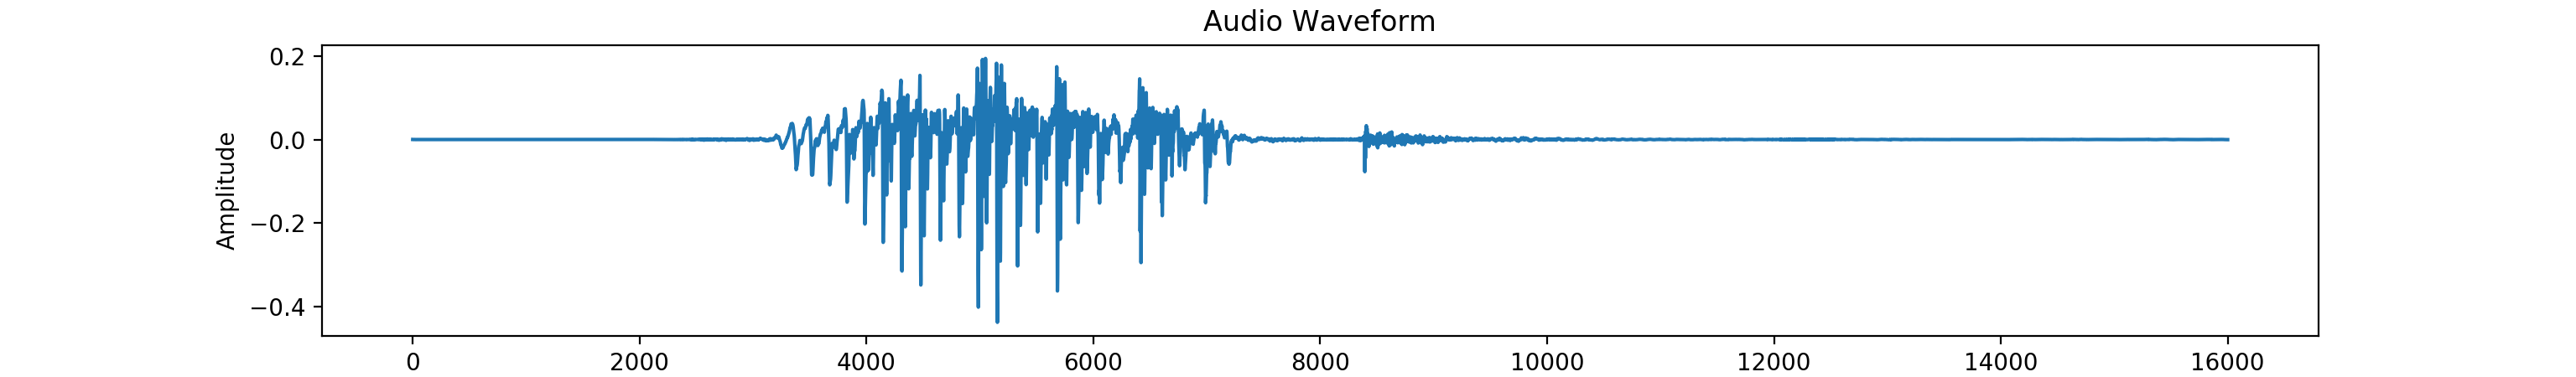
\includegraphics[width=\linewidth]{images/waveform-right}
    \caption{Audio waveform of utterance ``right''}
    \label{fig:wave_right}
  \end{subfigure}%
  \begin{subfigure}{.45\textwidth}
    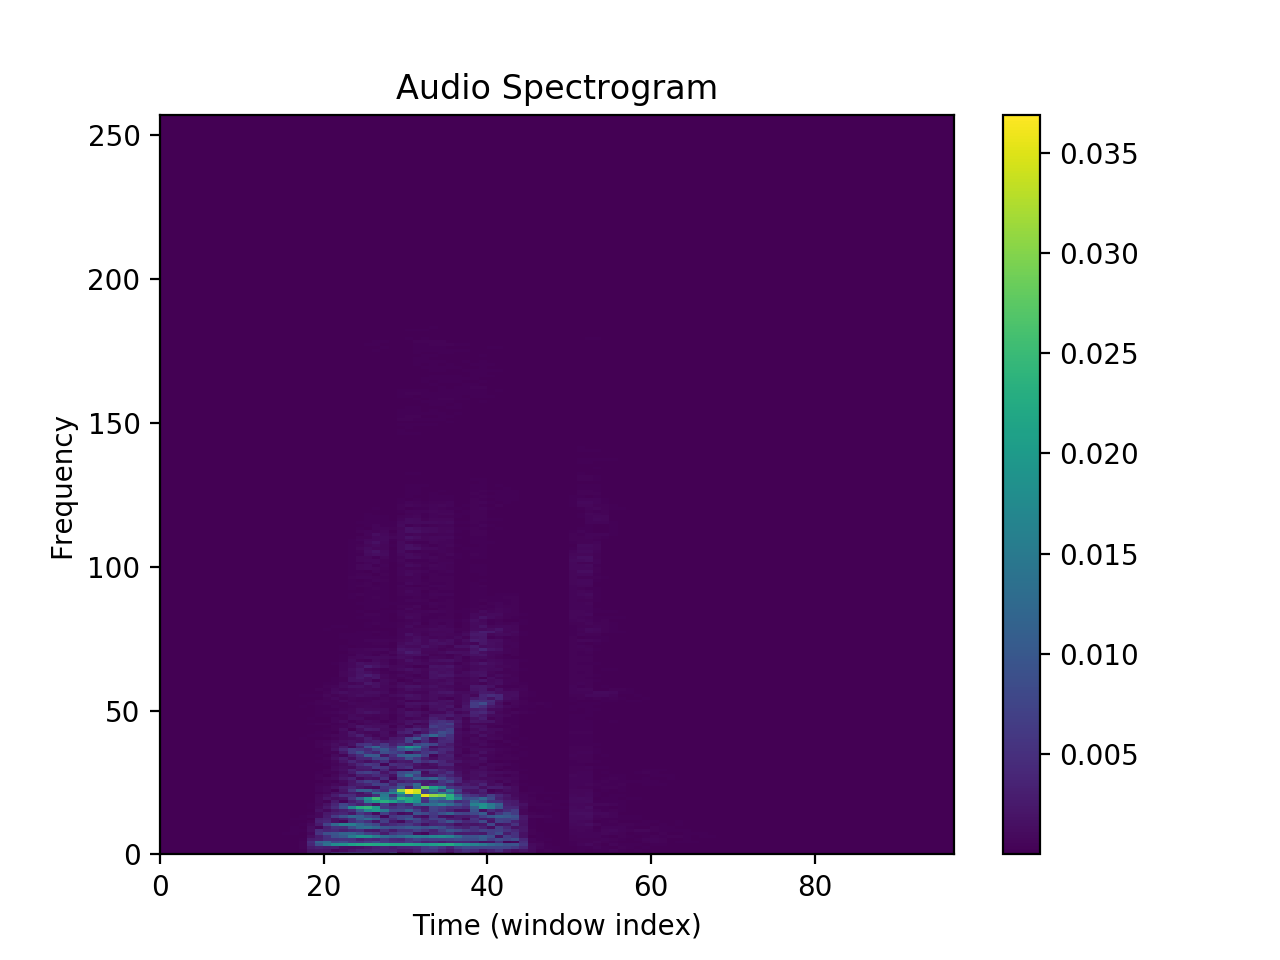
\includegraphics[width=0.75\linewidth]{images/spectrogram-right}
    \caption{Audio spectrogram of utterance ``right''}
    \label{fig:spec_right}
  \end{subfigure}
  \caption{Representations of audio data}
\end{figure}

Model evaluation was done with the use of spectrogram to
transform the audio waveform. The spectrogram computes the magnitude
of the short time Fourier transform of the 1D audio waveform over a
short window of the data. The window of the transform passes over the
waveform through time with some stride. This representation of the
data provides the magnitude of different frequencies that compose the
audio waveform during the time window that is under consideration. The
spectrogram of the utterance ``right'' is seen in figure
\ref{fig:spec_right}. The spectrogram shows that the waveform is
composed of large magnitudes of frequencies at the low end
corresponding to the word. For evaluation of the model without the use
of spectrograms as input data transformation, the audio waveform was
used keeping the sampling rate at 16KHz.

\section{ Methods }
As a simple baseline model, a simple multilayer convolutional neural
network (CNN) was evaluated[1]. The motivation behind a CNN network
architecture is to take advantage of the 2D nature of the spectrogram
of the sound wave. Since the spectrogram is two dimensional, a 2D
convolutional filter should be able to extract features from this
representation of the input. Coupled with this is the fairly
consistent size of the input audio waveform, and a CNN network can
take the spectrogram of an entire speech utterance as an input
image. The specific CNN model that was used for the baseline is a 4
layer CNN interleaved with 2x2 max pool layers\cite{oxerin-baseline}. The convolutional
layers all implement 3x3 filter kernels and contain power of two
multiples of 16 filters per layer (The layers from 1 to 4 contain
16, 32, 64, 128 filters respectively. These are then followed by 2
fully connected layers and finally a softmax output layer. The
baseline model is described in figure \ref{fig:baseline}. Also
evaluated are networks with time dimensional convolutions fed to a
recurrent LSTM layer. These would correspond to the more traditional
recurrent speech recognition networks.

\begin{figure}
  \begin{subfigure}{.45\textwidth}
    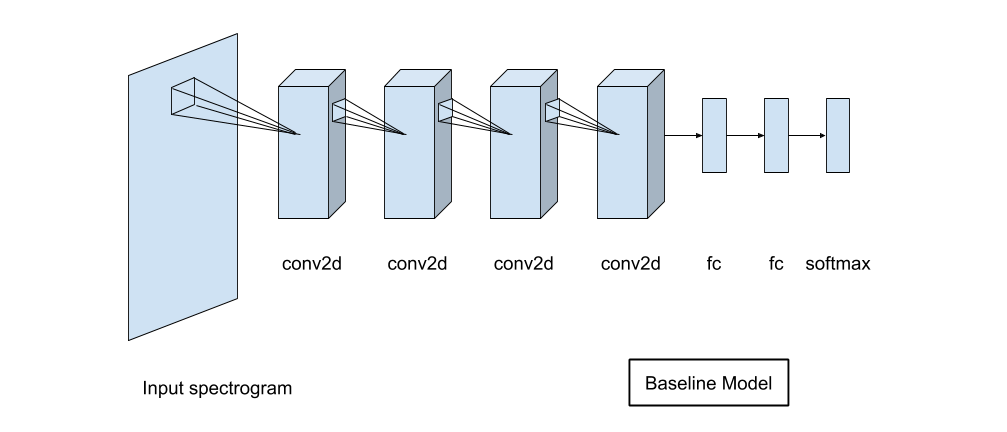
\includegraphics[width=\linewidth]{images/baseline}
    \caption{Baseline convolutional model}
    \label{fig:baseline}
  \end{subfigure}%
  \begin{subfigure}{.45\textwidth}
    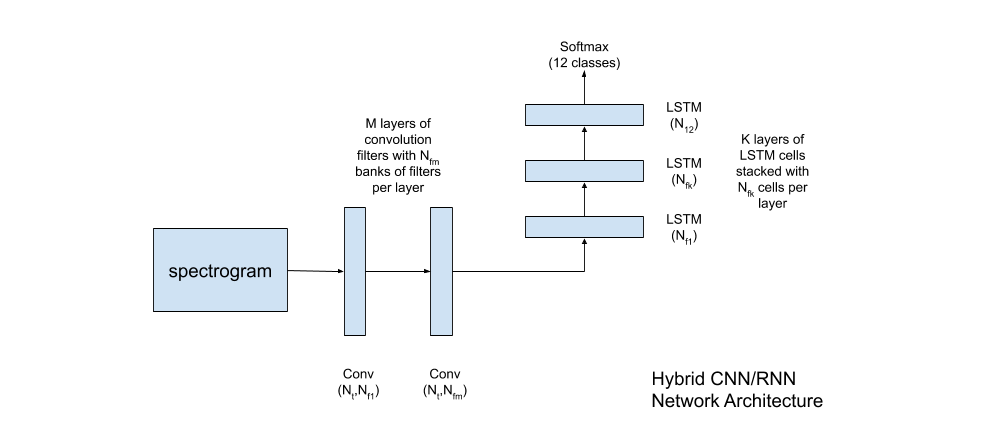
\includegraphics[width=\linewidth]{images/crnn}
    \caption{Convolutional-recurrent model}
    \label{fig:crnn}
  \end{subfigure}
  \caption{Model architectures evaluated}
\end{figure}

These two models are merged into a hybrid network (figure
\ref{fig:crnn}) taking the
advantages of both systems. At the end of the convolutional layers, we
are left with a time sequence of several frequency features for each
of the filter bank outputs. At this point, instead of performing a max
or average pooling step across all of the frequencies, we stack all of
the frequency and filter outputs for a point in time into a single
feature vector at that time point. This allow for keeping separate
features for the output of each filter bank to feed into the recurrent
layers following a fairly standard multi-layer recurrent
network. which feeds to a softmax output to determine the command
class.

The proposed network takes a batch of spectrograms of audio data, since
our data has been processed to all be of a fixed length at 16,000
samples. The input spectrogram contains 512 frequencies over a window
length of 512 samples of the audio waveform. The audio windows for spectral
transformation have a stride of 160 pixels (or 10ms) of audio. This
generates an input data set of 512 frequencies over 97 time samples of
data. This feeds multiple 2D convolutional and max pooling layers.

The convolutional layers successively perform 2D convolution on the
input. Following the convolution is a batch normalization layer to aid
in training. Before being fed into the next set of convolutional layer
there is a dropout layer to aid in reducing the variance of the
network. This is then fed into the activation layer which uses a
ReLU activation function. Finally, there is a max pooling step with a
2x2 window and a stride of 2 samples to produce the output of the
convolution layer. This set of layers are repeated with more filters
used in each layer. The convolutions will extract features in both the
time and frequency domains and look for certain patterns in the
data. The max pool step in each layer provides some level of
invariance in both time and frequency to account for variations in the
speed that the speaker is speaking and also the pitch of the
speaker. The multiple layers will extract larger and larger features
in the data where individual sounds uttered can vary in both time and
frequency due to the use of the max polling layers to aid in
robustness. Details are provided in figure \ref{fig:crnn-conv}.

The outputs of the convolutional portion of the network are then
flattened per time step and fed to one of more recurrent layers as
described in figure \ref{fig:crnn-lstm}. These
recurrent layers perform sequential modeling of the input data from
the convolutions over time. The LSTM layers use a hyperbolic tangent
activation function. The recurrent activation function is the hard
sigmoid function.

These recurrent layers allow us to process
the audio data over time without needing to have access to the entire
sample all at once. The advantage here is that we can continually feed
data into the recurrent network as we get more audio data which
overcomes the main drawback of the fully connected or convolutional
only network architectures. Beyond that, as we get more audio data
over time, we can only keep a window of convolutional results and add
to it as we get more raw data. We don't need to keep all of the raw
data to process, but rather only enough that we can generate new
convolutional results as needed. The output of the last LSTM layer
passes into a fully connected layer which generates a softmax output.

\begin{figure}
  \begin{subfigure}{.45\textwidth}
    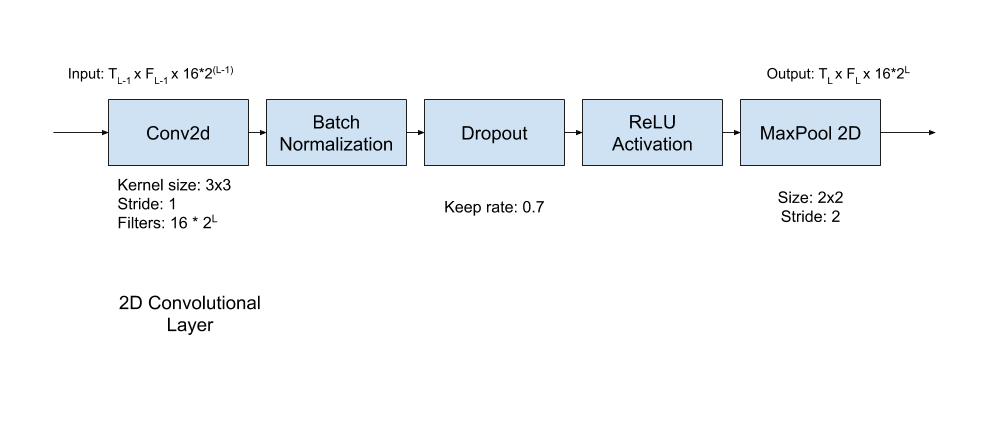
\includegraphics[width=\linewidth]{images/crnn-conv_layer}
    \caption{Convolutional layer detail}
    \label{fig:crnn-conv}
  \end{subfigure}%
  \begin{subfigure}{.45\textwidth}
    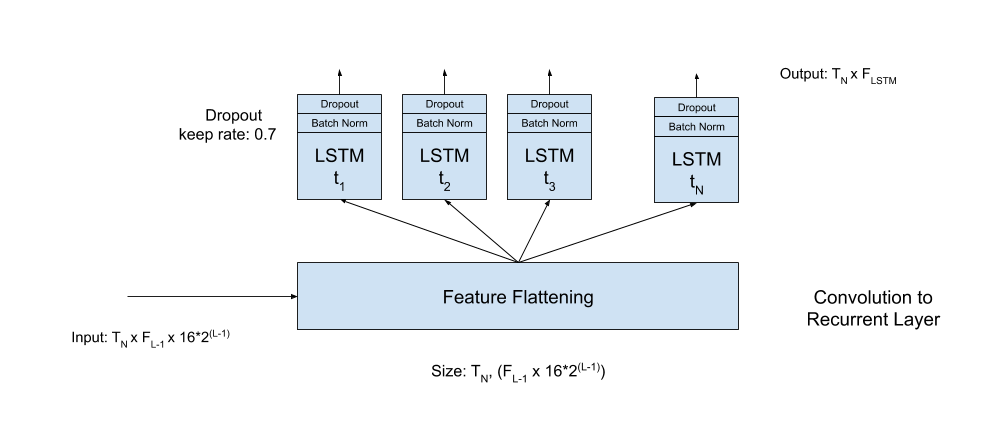
\includegraphics[width=\linewidth]{images/crnn-lstm_layer}
    \caption{Convolutional to recurrent layer}
    \label{fig:crnn-lstm}
  \end{subfigure}
  \caption{Details of proposed model layers}
\end{figure}

We also explored having the network learn the basis function for a
spectral transform which is currently performed by the short-time
Fourier Transform to compute the spectrogram which would allow our
system to be a true end-to-end system where it would be fed only
samples of audio. This is accomplished by multiple filter banks of a
single one dimensional convolution
layer in the network at the input which would produce an output like the
spectrogram but projecting a window of data from the audio waveform
into a learned set of basis functions instead of sine and cosine waves.

The loss for the network is the categorical loss function for single
class selection based on one-hot encoding. The entire network is
trained using the Adam optimization algorithm using a learning rate of
0.001 and a learning rate decay of 0.0001.

Our models were developed in Python with the Keras framework running
on a single the TensorFlow backend. Experiments were run on Google
Cloud using the Deep Learning VM with an NVidia Tesla K80 GPU
attached. The system could train a 2 million parameter model at
approximately 500ms per step. This results in training our model with
3 conv2d layers and 2 recurrent layers with batch normalization,
dropout, and learning rate decay for 20 epochs in approximately 75
minutes. Code is available from GitHub:
\url{https://github.com/tomkarpati/cs230.git}

\section{Experiments/Results/Discussion}
Our baseline model produced fairly decent results in line with our
expectations. The model produced 80\% accuracy on the test set
provided with the dataset. While the results were reassuring, the
model still suffered from the drawbacks outlined above. The second of
our models was the recurrent network with non-pooling single
dimensional convolution. While this model addressed the drawbacks of
the convolution only baseline model, this model produced worse results
in the simple case. The 1D convolutional model was tuned to get an
idea of the impact from different parameters.

A summary of results of tuning the 1D convolutional baseline mode are
outlined in table \cite{tab:summary-results}. The largest impact was
provided by both an increase in the number of convolutional layers and
the number of recurrent layers as expected. The training accuracy of
the model increased from a single convolutional layer to 3
convolutional layers and 1 LSTM layer to 3 LSTM layers. While the
training accuracy of the model was fairly high, the model showed high
variance as seen by the much lower accuracy number on the validation
data without dropout. A dropout keep rate of 0.7
produced good results, but a lower rate appeared to spread the
features too much across the weights between the layers. For the 1D
convolutional model, the larger kernel sizes produced better
results. To counteract the noise in the loss functions
as the loss converged to zero, we introduced learning rate decay and a
value of 0.0001 produced good results.

Our two dimensional convolutional model was also tuned across the same
lines (cite{tab:summary-results}). Again we increased layers to 3
convolutional layers and 3 recurrent layers. Training speed was
increased with batch normalization and variance reduced with dropout
at a keep rate of 0.7. With the two dimensional convolutional layers,
we noticed a decease in accuracy with the increase in 2D convolutional
kernel sizes and strides. Additionally, increases in the number of
hidden nodes in our LSTM layers marginally increased our training
accuracy, but this did not translate to any increase in our validation
results indicating overfitting of our data. In addition, we also
looked at effect of varying the FFT parameters that were used to feed
the spectrograms to the network. Decreasing the FFT length and window
size over the values 512, 256, 128, and 64 did not produce any better
results as the FFT got smaller, however the number of parameters did
get smaller resulting in a smaller and faster model
computationally and less required memory.

\begin{table}
  \resizebox{\textwidth}{!} {
    \begin{tabular} { |m{2.5cm}|c|c|c|c|c|m{5cm}|c|c|c|c| }
      \hline
      Architecture & \multicolumn{3}{|c|}{Convolutional Kernel} &
      \multicolumn{2}{|c|}{Recurrent} & Other &
      \multicolumn{2}{|c|}{Parameters} & \multicolumn{2}{|c|}{Accuracy} \\
      \hline
      & Size & Stride & \# Layers &
      \# Cells & \# Layers & &
      Total & Trainable & Train & Validation \\ \hline
      \hline
      Baseline & 3 & 1 & 4 &
      - & - & Dropout=0.5, FC (N=128), Activation=ELU, Global pooling &
      - & - & 0.8066 & 0.8073 \\ \hline
      \hline
      Keras Baseline & 3 & 1 & 4 &
      - & - & Dropout=0.5, FC (N=128), Activation=ELU, Flattening &
      2,048K & 2,048K & 0.9805 & 0.0206 \\ \hline
      \hline
      Conv1d LSTM & 3 & 1 & 2 &
      128 & 1 & Dropout=0.7, lr\_decay=0.0001 &
      383K & 382K & 0.9005 & 0.9081 \\ \hline
      \hline
      conv2d LSTM & 3 & 1 & 3 &
      128 & 3 & Dropout=0.7, lr\_decay=0.0001 &
      1,439K & 1,437K & 0.9860 & 0.9459 \\ \hline
      \hline
      conv2d LSTM & 3 & 1 & 3 &
      256 & 3 & Dropout=0.7, lr\_decay=0.0001 &
      3,509K & 3,507K & 0.9875 & 0.9385 \\ \hline
      conv2d LSTM & 3 & 1 & 3 &
      384 & 3 & Dropout=0.7, lr\_decay=0.0001 &
      6,235K & 6,232K & 0.9892 & 0.9135 \\ \hline
      \hline
      conv2d LSTM & 3 & 1 & 3 &
      128 & 3 & Dropout=0.7, lr\_decay=0.0001,
      fft (l=256,s=128) &
      914K & 913K & 0.9863 & 0.9029 \\ \hline
      conv2d LSTM & 3 & 1 & 3 &
      128 & 3 & Dropout=0.7, lr\_decay=0.0001,
      fft(l=128,s=64) &
      652K & 651K & 0.9839 & 0.9319 \\ \hline
      conv2d LSTM & 3 & 1 & 3 &
      128 & 3 & Dropout=0.7, lr\_decay=0.0001,
      fft(l=64,s=32) &
      521K & 520K & 0.9831 & 0.9272 \\ \hline
    \end{tabular}
  }
  \caption{Summary experimental results}
  \label{tab:summary-results}
\end{table}
Finally, we attempted to have the network learn basis functions for
the initial raw audio preprocessing. The addition of the one
dimensional convolutional layer resulted in our model becoming
untrainable. Our training and validation set accuracies were not able
to increase beyond about 60\%. We started with a 1D convolutional
kernel of 512 samples and stride of 256 samples. The trainability of
our model didn't see any improvement as the size of the initial 1D
kernel was decrease through 256, 128, and 64 samples (with 1/2 FFT
with window stride through the audio data). The initial basis function
mapping appeared to be too large for the model to be able to minimize
the loss functional effectively.

\section{Conclusion/Future Work }
We found that the our hybrid convolutional and recurrent network
produced good results on our dataset but we believe it would be better
suited to command detection in the real world than some of the other 2D
convolutional and fully connected networks that we had looked at due
to the use of the unidirectional recurrent cells due to
some invariance on both the time and frequency domains. Our attempts
to learn new basis functions to replace the initial short-time Fourier
transform preprocessing step were unproductive. Additional work would
involve more testing of utterances of commands from other speakers
that are not used in either the training or validation steps to
determine accuracy to commands spoken by users who have never been
seen before. Finally, additional work would be to implement a simple
preprocessing step to differentiate any utterances from background
noise to initially screen out background noise, and reduce the overall
computation that the system performs over time, to just the time when
the system can determine that it actually needs to be paying attention.

\bibliography{cs230}{}
\bibliographystyle{plain}

\newpage

\begin{table}
  \resizebox{\textwidth}{!} {
    \begin{tabular} { |m{2.5cm}|c|c|c|c|c|m{3.5cm}|c|c|c|c| }
      \hline
      Architecture & \multicolumn{3}{|c|}{Convolutional Kernel} &
      \multicolumn{2}{|c|}{Recurrent} & Other &
      \multicolumn{2}{|c|}{Parameters} & \multicolumn{2}{|c|}{Accuracy} \\
      \hline
      & Size & Stride & \# Layers &
      \# Cells & \# Layers & &
      Total & Trainable & Train & Validation \\ \hline
      \hline
      Baseline & 3 & 1 & 4 &
      - & - & Batch Norm, Dropout=0.5, FC (N=128), Activation=ELU, Global pooling &
      - & - & 0.8066 & 0.8073 \\ \hline
      \hline
      Keras Baseline & 3 & 1 & 4 &
      - & - & Batch Norm, Dropout=0.5, FC (N=128), Activation=ELU, Flattening &
      2,048K & 2,048K & 0.9805 & 0.0206 \\ \hline
      \hline
      Conv1d LSTM & 3 & 1 & 1 &
      128 & 1 & No Batch Norm, No Dropout &
      88K & 88K & 0.7061 & 0.7651 \\ \hline
      Conv1d LSTM & 3 & 1 & 2 &
      128 & 2 & No Batch Norm, No Dropout &
      219K & 219K & 0.7940 & 0.7924 \\ \hline
      Conv1d LSTM & 3 & 1 & 1 &
      128 & 1 & Batch Norm, No Dropout &
      89K & 88K & 0.9482 & 0.8956 \\ \hline
      Conv1d LSTM & 3 & 1 & 1 &
      128 & 2 & Batch Norm, No Dropout &
      221K & 220K & 0.9530 & 0.8726 \\ \hline
      Conv1d LSTM & 3 & 1 & 2 &
      128 & 1 & Batch Norm, No Dropout &
      99K & 98K & 0.9497 & 0.9028 \\ \hline
      Conv1d LSTM & 3 & 1 & 2 &
      128 & 2 & Batch Norm, No Dropout &
      231K & 230K & 0.9422 & 0.8850 \\ \hline
      Conv1d LSTM & 3 & 1 & 3 &
      128 & 3 & Batch Norm, No Dropout &
      388K & 386K & 0.9610 & 0.8898 \\ \hline
      \hline
      Conv1d LSTM & 5 & 3 & 2 &
      128 & 3 & Batch Norm, No Dropout &
      374K & 373K & 0.9709 & 0.8945 \\ \hline
      Conv1d LSTM & 7 & 3 & 2 &
      128 & 3 & Batch Norm, No Dropout &
      383K & 382K & 0.9706 & 0.8982 \\ \hline
      Conv1d LSTM & 15 & 3 & 2 &
      128 & 3 & Batch Norm, No Dropout &
      421K & 419K & 0.9648 & 0.8942 \\ \hline
      \hline
      Conv1d LSTM & 3 & 1 & 2 &
      128 & 1 & Batch Norm, Dropout=0.5 &
      100K & 99K & 0.9041 & 0.8470 \\ \hline
      Conv1d LSTM & 3 & 1 & 2 &
      128 & 1 & Batch Norm, Dropout=0.7 &
      100K & 99K & 0.9631 & 0.8923 \\ \hline
      Conv1d LSTM & 3 & 1 & 3 &
      128 & 3 & Batch Norm, Dropout=0.5 &
      388K & 386K & 0.9107 & 0.8395 \\ \hline
      Conv1d LSTM & 3 & 1 & 3 &
      128 & 3 & Batch Norm, Dropout=0.7 &
      388K & 386K & 0.9445 & 0.8480 \\ \hline
      \hline
      Conv1d LSTM & 7 & 3 & 2 &
      128 & 3 & Batch Norm, Dropout=0.7, lr\_decay=0.0 &
      383K & 382K & 0.8957 & 0.8953 \\ \hline
      Conv1d LSTM & 7 & 3 & 2 &
      128 & 3 & Batch Norm, Dropout=0.7, lr\_decay=0.001 &
      383K & 382K & 0.8684 & 0.9060 \\ \hline
      Conv1d LSTM & 3 & 1 & 2 &
      128 & 1 & Batch Norm, Dropout=0.7, lr\_decay=0.0001 &
      383K & 382K & 0.9005 & 0.9081 \\ \hline
      \hline
      conv2d LSTM & 3 & 1 & 2 &
      128 & 1 & Batch Norm &
      1,138K & 1,138K & 0.9822 & 0.8907 \\ \hline
      conv2d LSTM & 3 & 1 & 3 &
      128 & 2 & Batch Norm &
      1,306K & 1,305K & 0.9862 & 0.9425 \\ \hline
      conv2d LSTM & 3 & 1 & 3 &
      128 & 3 & Batch Norm &
      1,439K & 1,437K & 0.9822 & 0.9347 \\ \hline
      \hline
      conv2d LSTM & 3 & 1 & 3 &
      128 & 3 & Batch Norm, Dropout=0.7, lr\_decay=0.0 &
      1,439K & 1,437K & 0.9779 & 0.9525 \\ \hline
      conv2d LSTM & 3 & 1 & 3 &
      128 & 3 & Batch Norm, Dropout=0.7, lr\_decay=0.001 &
      1,439K & 1,437K & 0.9824 & 0.8756 \\ \hline
      conv2d LSTM & 3 & 1 & 3 &
      128 & 3 & Batch Norm, Dropout=0.7, lr\_decay=0.0001 &
      1,439K & 1,437K & 0.9860 & 0.9459 \\ \hline
      \hline
      conv2d LSTM & 5 & 3 & 3 &
      128 & 3 & Batch Norm, Dropout=0.7, lr\_decay=0.0001 &
      464K & 463K & 0.8308 & 0.8536 \\ \hline
      conv2d LSTM & 7 & 3 & 3 &
      128 & 3 & Batch Norm, Dropout=0.7, lr\_decay=0.0001 &
      526K & 525K & 0.8737 & 0.8672 \\ \hline
      \hline
      conv2d LSTM & 3 & 1 & 3 &
      256 & 3 & Batch Norm, Dropout=0.7, lr\_decay=0.0001 &
      3,509K & 3,507K & 0.9875 & 0.9385 \\ \hline
      conv2d LSTM & 3 & 1 & 3 &
      384 & 3 & Batch Norm, Dropout=0.7, lr\_decay=0.0001 &
      6,235K & 6,232K & 0.9892 & 0.9135 \\ \hline
      \hline
      conv2d LSTM & 3 & 1 & 3 &
      128 & 3 & Batch Norm, Dropout=0.7, lr\_decay=0.0001,
      fft(l=256,s=128) &
      914K & 913K & 0.9863 & 0.9029 \\ \hline
      conv2d LSTM & 3 & 1 & 3 &
      128 & 3 & Batch Norm, Dropout=0.7, lr\_decay=0.0001,
      fft(l=128,s=64) &
      652K & 651K & 0.9839 & 0.9319 \\ \hline
      conv2d LSTM & 3 & 1 & 3 &
      128 & 3 & Batch Norm, Dropout=0.7, lr\_decay=0.0001,
      fft(l=64,s=32) &
      521K & 520K & 0.9831 & 0.9272 \\ \hline
      
    \end{tabular}
  }
\end{table}

\end{document}
